\chapter{The emerging field of graph signal processing}
Nowadays huge amounts of data are collected every day, from engineering sciences to our personal data regarding health monitoring, to financial data or political influences. The analysis and the process of these huge datasets has become a non indifferent challenge, since, in fact, data tends to reside on complex and irregular structures, which progressively required the introduction of innovative approaches to better handle and utilize them. \cite{Ortega2017} \cite{Sandry}

One of the central entities we will use in this work is the concept of \textit{graph signal}. Graphs are generic data representation structures, which are useful in a great variety of fields and applications for everyday life and technology in general. These structures are composed by two main elements: the nodes and the edges; the former are a set of points, identifying an aspect of the graph structure itself, while the latter are connections between the nodes. Several structures we can encounter in natural entities and abstract constructions can be represented by a graph structure, and when we associate values to their set of nodes and edges we obtain a graph signal. To be specific, a graph signal is seen as a finite collection of samples located at each node in the structure and which are interconnected among themselves through the edges, to which we can associate numerical values representing the weights of the connections. The metric for these weights is not unique, as it depends on which relation between the nodes we are looking at: a typical metric for graph weights may be, for example, inversely proportional to the distance (physical or not) between two different nodes, but other options are possible.

As previously mentioned, graph structures appear to be significantly helpful when they are used to represent signals and their applications are the most varied: we could focus on transportation networks, where we could want to work with data describing human migration patterns or trade goods; we could also apply graph theory over social networks, in which users can be seen, for example, as our nodes while their connections to friends are our edges. \cite{Ortega2017} Brain imaging is another interesting application of graph signals: through it we could infer the inner structure of some regions of the brain, in a way that permits us to better understand physiological dynamics.  \cite{Shuman2013} We could go on listing a considerable amount of valuable applications, from genetic and biochemical research to fundamental physical experiments; what these big amounts of data have in common is the fact that their complex inner structure makes it difficult to apply most of the well-known tools, like \gls{pca}, spectral analysis or \gls{svd}, without redefining the signal structure. \cite{Sandry}

\section{Mathematical description of the graph structure}
In the field of \gls{gsp}, spectral graph theory plays an important role, it focuses on analysing, constructing and manipulating graphs and makes uses of well know tools and concepts as frequency spectrum and the graph Fourier transform. In our work, the signals we are considering are defined on an undirected, connected, weighted graph $\mathcal{G} = \{ \mathcal{V}, \varepsilon, W\}$ consisting on a finite set of vertices $\mathcal{V}$ with $|\mathcal{V}| = N$, a set of edges $\varepsilon$ and a weighted adjacency matrix $\mathcal{W}$. The adjacency matrix contains the information of the connections between two nodes: if an edge $e$ is present between two vertices $i$ and $j$, then the entry $W_{i,j}$ represents the weight of that edge, while if there is no connection between two nodes, the value of the edge is null ($W_{i,j} = 0$). Moreover, if the graph was not connected and had K connected components, then we could decompose the graph signal over $\mathcal{G}$ into M sections which can be processed each one independently of the other.

Over this structure, we can then spread the signal we need to analyse: to be precise, a signal or function $f: \mathcal{V} \to \R$ defined on the vertices of our graph, can be described as a vector $f \in \R^N$ that has the signal value at the $i^{th}$ vertex in $\mathcal{V}$ as the $i^{th}$ component of the vector $f$. \autoref{fig:sampleGraph} shows an example of graph signal: the colours of the vertices represents the values the signal has on them.

\begin{figure}
  \centering
  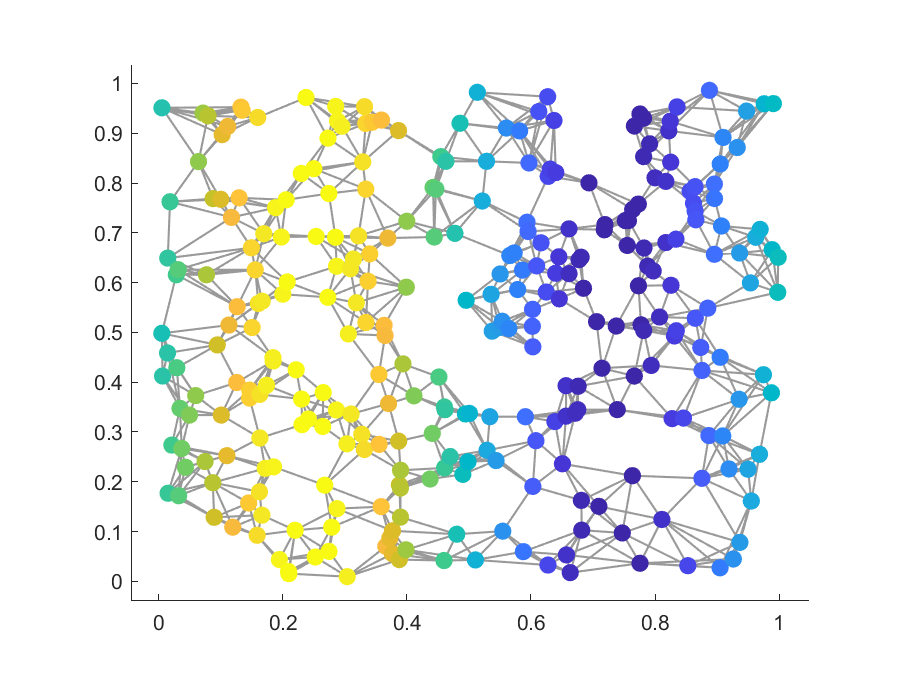
\includegraphics[width = .7\textwidth]{sampleGraph2.eps}
  \caption{Random sensor graph}
  \label{fig:sampleGraph}
\end{figure}
\section{the inverse covariance matrix}
\cri{Vedere se aggiungere o meno questa sezione}

\subsubsection{The graph Laplacian}
\label{sec:graph laplacian}
To go from the graph vertex domain (which plays the same role of the time domain in the classical signal processing theory) to the spectral domain the \textit{graph Laplacian operator}, or \textit{Combinatorial graph Laplacian}, has been introduced, which is defined as $L := D - W$, where $D$ represents a diagonal matrix whose  $i^{th}$ diagonal element is equal to the sum of weights of all the edges incident to the vertex $i$. This entity is a difference operator, since it satisfies the condition:
\begin{equation}
((L f)(i) = \sum_{j \in \mathcal{N}_i} W_{i,j}[f(i) - f(j)]
\end{equation}
The element $\mathcal{N}_i$ represents the set of vertices connected to vertex $i$ by an edge.

From its definition, the graph Laplacian $L$ is a real symmetric matrix, thus it has a complete set of orthonormal eigenvectors, here denoted by $\{u_l\}_{l=0,1,\dots,N-1}$, to which real and non-negative eigenvalues are associated ($\{\lambda_l\}_{l=0,1,\dots,N-1}$). Together with the eigenvectors, they satisfy the condition:
\begin{equation}
L u_l = \lambda_l u_l, \text{   for  } l = 0,1,\dots,N-1
\end{equation}
In the eigenvalues set, the one corresponding to $0$ has a multiplicity equal to the number of connected components of the graph; from this, since we are considering only connected graphs, we can assume the Laplacian eigenvalues have the distribution: $0 = \lambda_0 < \lambda_1 \leq \lambda_2 \dots \leq \lambda_{N-1} = \lambda_{max}$ and, of course, the set $\sigma(L) = \{\lambda_0, \lambda_1,\dots,\lambda_{N-1}\}$ is the entire spectrum of our signal.

Eigenvalues and eigenvectors are then used to build up the graph version of a well known and useful transform, which is the \textit{classical Fourier Transform} and that we recall here being defined as:
\begin{equation}
\hat{f}(\xi) = \langle f, e^{2\pi i \xi t}\rangle = \int_{\R} f(t)e^{-2\pi i \xi t} dt
\end{equation}
and that we can see as the expansion of a function $f$ in terms of the complex exponentials, elements which represent the eigenfunctions of the one-dimensional Laplace operator:
\begin{equation}
-\Delta(e^{2\pi i \xi t}) = -\frac{\partial^2}{\partial t^2}e^{2\pi i \xi t} = (2\pi\xi)^2e^{2\pi i \xi t}
\end{equation}
From the observation of the classical Fourier Transform, we can analogously define the \textit{Graph Fourier Transform} $\hat{f}$ of any function $f \in \R^N$ on the vertices of $\mathcal{G}$ as the expansion of $f$ in terms of the eigenvectors of the graph Laplacian \cite{Shuman2013}:
\begin{equation}
\hat{f}(\lambda_l) = \langle f, u_l \rangle = \sum^{N}_{i=1}f(i)u_l*(i)
\end{equation}
while, at the same time, the \textit{inverse Graph Fourier Transform} is given by:
\begin{equation}
f(i) = \sum^{N-1}_{l = 0}\hat{f}(\lambda_l)u_l(i)
\end{equation}
